\begin{figure}[tbp]
\centering
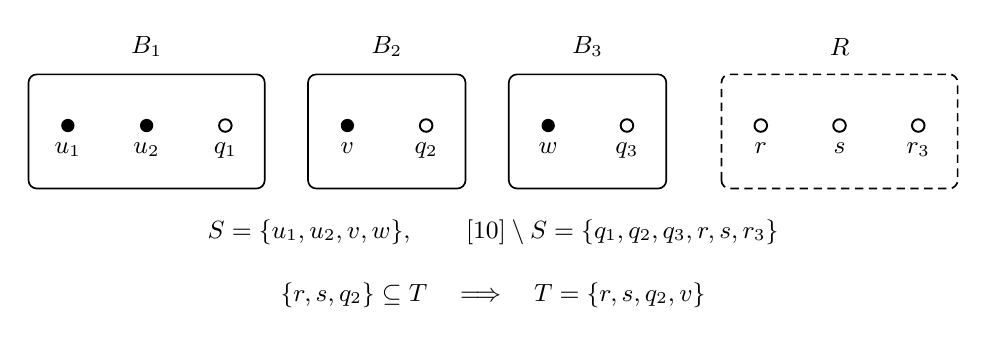
\begin{tikzpicture}[
  x=1cm,y=1cm,font=\small,
  present/.style={circle,fill=black,inner sep=1.7pt},
  omitted/.style={circle,draw=black,fill=white,inner sep=1.6pt,line width=.7pt},
  every path/.style={line width=.6pt}
]
\draw[rounded corners=3pt] (0,.35) rectangle (3,1.8);
\draw[rounded corners=3pt] (3.55,.35) rectangle (5.55,1.8);
\draw[rounded corners=3pt] (6.1,.35) rectangle (8.1,1.8);
\draw[rounded corners=3pt,densely dashed] (8.8,.35) rectangle (11.8,1.8);
\node at (1.5,2.15) {$B_1$};
\node at (4.55,2.15) {$B_2$};
\node at (7.1,2.15) {$B_3$};
\node at (10.3,2.15) {$R$};
\node[present,label=below:$u_1$] at (.5,1.15) {};
\node[present,label=below:$u_2$] at (1.5,1.15) {};
\node[omitted,label=below:$q_1$] at (2.5,1.15) {};
\node[present,label=below:$v$] at (4.05,1.15) {};
\node[omitted,label=below:$q_2$] at (5.05,1.15) {};
\node[present,label=below:$w$] at (6.6,1.15) {};
\node[omitted,label=below:$q_3$] at (7.6,1.15) {};
\node[omitted,label=below:$r$] at (9.3,1.15) {};
\node[omitted,label=below:$s$] at (10.3,1.15) {};
\node[omitted,label=below:$r_3$] at (11.3,1.15) {};
\node at (5.9,-.2) {$S=\{u_1,u_2,v,w\},\qquad [10]\setminus S=\{q_1,q_2,q_3,r,s,r_3\}$};
\node at (5.9,-1) {$\{r,s,q_2\}\subseteq T\quad\Longrightarrow\quad T=\{r,s,q_2,v\}$};
\end{tikzpicture}
\caption{The only remaining block sizes are $3,2,2$, with three
labels in $R$ outside the blocks. Filled dots are the vertices of the
fixed tetrahedron $S$; the omitted block elements are $q_1,q_2,q_3$.
Every tetrahedron must contain two vertices of one block. After
relabeling the two-element blocks, the final argument selects a triangle
$\{r,s,q_2\}$ with $r,s\in R$. Its only possible tetrahedral extension
is obtained by adjoining $v$, contradicting the two required extensions.}
\label{fig:partner-blocks}
\end{figure}
